\documentclass[12pt,]{article}
%DIF LATEXDIFF DIFFERENCE FILE
%DIF DEL /Users/mkdoherty/Documents/Janssen/Doherty_CDprediction_mBio_2017/submission/Doherty_CDprediciton_mBio_2017_finaldraft_nographics.tex   Mon Nov 20 14:26:06 2017
%DIF ADD /Users/mkdoherty/Documents/Janssen/Doherty_CDprediction_mBio_2017/submission/Doherty_CDprediciton_mBio_2017_AddRevComm_nographics.tex   Thu Feb  1 17:04:07 2018
\usepackage{lmodern}
\usepackage{amssymb,amsmath}
\usepackage{ifxetex,ifluatex}
\usepackage{fixltx2e} % provides \textsubscript
\ifnum 0\ifxetex 1\fi\ifluatex 1\fi=0 % if pdftex
  \usepackage[T1]{fontenc}
  \usepackage[utf8]{inputenc}
\else % if luatex or xelatex
  \ifxetex
    \usepackage{mathspec}
  \else
    \usepackage{fontspec}
  \fi
  \defaultfontfeatures{Ligatures=TeX,Scale=MatchLowercase}
\fi
% use upquote if available, for straight quotes in verbatim environments
\IfFileExists{upquote.sty}{\usepackage{upquote}}{}
% use microtype if available
\IfFileExists{microtype.sty}{%
\usepackage{microtype}
\UseMicrotypeSet[protrusion]{basicmath} % disable protrusion for tt fonts
}{}
\usepackage[margin=1.0in]{geometry}
\usepackage{hyperref}
\hypersetup{unicode=true,
            pdftitle={Fecal microbiota signatures are associated with response to Ustekinumab therapy among Crohn's Disease patients},
            pdfborder={0 0 0},
            breaklinks=true}
\urlstyle{same}  % don't use monospace font for urls
\usepackage{graphicx,grffile}
\makeatletter
\def\maxwidth{\ifdim\Gin@nat@width>\linewidth\linewidth\else\Gin@nat@width\fi}
\def\maxheight{\ifdim\Gin@nat@height>\textheight\textheight\else\Gin@nat@height\fi}
\makeatother
% Scale images if necessary, so that they will not overflow the page
% margins by default, and it is still possible to overwrite the defaults
% using explicit options in \includegraphics[width, height, ...]{}
\setkeys{Gin}{width=\maxwidth,height=\maxheight,keepaspectratio}
\IfFileExists{parskip.sty}{%
\usepackage{parskip}
}{% else
\setlength{\parindent}{0pt}
\setlength{\parskip}{6pt plus 2pt minus 1pt}
}
\setlength{\emergencystretch}{3em}  % prevent overfull lines
\providecommand{\tightlist}{%
  \setlength{\itemsep}{0pt}\setlength{\parskip}{0pt}}
\setcounter{secnumdepth}{0}
% Redefines (sub)paragraphs to behave more like sections
\ifx\paragraph\undefined\else
\let\oldparagraph\paragraph
\renewcommand{\paragraph}[1]{\oldparagraph{#1}\mbox{}}
\fi
\ifx\subparagraph\undefined\else
\let\oldsubparagraph\subparagraph
\renewcommand{\subparagraph}[1]{\oldsubparagraph{#1}\mbox{}}
\fi

%%% Use protect on footnotes to avoid problems with footnotes in titles
\let\rmarkdownfootnote\footnote%
\def\footnote{\protect\rmarkdownfootnote}

%%% Change title format to be more compact
\usepackage{titling}

% Create subtitle command for use in maketitle
\newcommand{\subtitle}[1]{
  \posttitle{
    \begin{center}\large#1\end{center}
    }
}

\setlength{\droptitle}{-2em}
  \title{Fecal microbiota signatures are associated with response to Ustekinumab
therapy among Crohn's Disease patients}
  \pretitle{\vspace{\droptitle}\centering\huge}
  \posttitle{\par}
  \author{}
  \preauthor{}\postauthor{}
  \date{}
  \predate{}\postdate{}

\usepackage{setspace}
\doublespacing
\usepackage{lineno}
\linenumbers
\renewcommand{\familydefault}{\sfdefault}
\usepackage{graphicx}
%DIF PREAMBLE EXTENSION ADDED BY LATEXDIFF
%DIF UNDERLINE PREAMBLE %DIF PREAMBLE
\RequirePackage[normalem]{ulem} %DIF PREAMBLE
\RequirePackage{color}\definecolor{RED}{rgb}{1,0,0}\definecolor{BLUE}{rgb}{0,0,1} %DIF PREAMBLE
\providecommand{\DIFaddtex}[1]{{\protect\color{blue}\uwave{#1}}} %DIF PREAMBLE
\providecommand{\DIFdeltex}[1]{{\protect\color{red}\sout{#1}}}                      %DIF PREAMBLE
%DIF SAFE PREAMBLE %DIF PREAMBLE
\providecommand{\DIFaddbegin}{} %DIF PREAMBLE
\providecommand{\DIFaddend}{} %DIF PREAMBLE
\providecommand{\DIFdelbegin}{} %DIF PREAMBLE
\providecommand{\DIFdelend}{} %DIF PREAMBLE
%DIF FLOATSAFE PREAMBLE %DIF PREAMBLE
\providecommand{\DIFaddFL}[1]{\DIFadd{#1}} %DIF PREAMBLE
\providecommand{\DIFdelFL}[1]{\DIFdel{#1}} %DIF PREAMBLE
\providecommand{\DIFaddbeginFL}{} %DIF PREAMBLE
\providecommand{\DIFaddendFL}{} %DIF PREAMBLE
\providecommand{\DIFdelbeginFL}{} %DIF PREAMBLE
\providecommand{\DIFdelendFL}{} %DIF PREAMBLE
%DIF HYPERREF PREAMBLE %DIF PREAMBLE
\providecommand{\DIFadd}[1]{\texorpdfstring{\DIFaddtex{#1}}{#1}} %DIF PREAMBLE
\providecommand{\DIFdel}[1]{\texorpdfstring{\DIFdeltex{#1}}{}} %DIF PREAMBLE
\newcommand{\DIFscaledelfig}{0.5}
%DIF HIGHLIGHTGRAPHICS PREAMBLE %DIF PREAMBLE
\RequirePackage{settobox} %DIF PREAMBLE
\RequirePackage{letltxmacro} %DIF PREAMBLE
\newsavebox{\DIFdelgraphicsbox} %DIF PREAMBLE
\newlength{\DIFdelgraphicswidth} %DIF PREAMBLE
\newlength{\DIFdelgraphicsheight} %DIF PREAMBLE
% store original definition of \includegraphics %DIF PREAMBLE
\LetLtxMacro{\DIFOincludegraphics}{\includegraphics} %DIF PREAMBLE
\newcommand{\DIFaddincludegraphics}[2][]{{\color{blue}\fbox{\DIFOincludegraphics[#1]{#2}}}} %DIF PREAMBLE
\newcommand{\DIFdelincludegraphics}[2][]{% %DIF PREAMBLE
\sbox{\DIFdelgraphicsbox}{\DIFOincludegraphics[#1]{#2}}% %DIF PREAMBLE
\settoboxwidth{\DIFdelgraphicswidth}{\DIFdelgraphicsbox} %DIF PREAMBLE
\settoboxtotalheight{\DIFdelgraphicsheight}{\DIFdelgraphicsbox} %DIF PREAMBLE
\scalebox{\DIFscaledelfig}{% %DIF PREAMBLE
\parbox[b]{\DIFdelgraphicswidth}{\usebox{\DIFdelgraphicsbox}\\[-\baselineskip] \rule{\DIFdelgraphicswidth}{0em}}\llap{\resizebox{\DIFdelgraphicswidth}{\DIFdelgraphicsheight}{% %DIF PREAMBLE
\setlength{\unitlength}{\DIFdelgraphicswidth}% %DIF PREAMBLE
\begin{picture}(1,1)% %DIF PREAMBLE
\thicklines\linethickness{2pt} %DIF PREAMBLE
{\color[rgb]{1,0,0}\put(0,0){\framebox(1,1){}}}% %DIF PREAMBLE
{\color[rgb]{1,0,0}\put(0,0){\line( 1,1){1}}}% %DIF PREAMBLE
{\color[rgb]{1,0,0}\put(0,1){\line(1,-1){1}}}% %DIF PREAMBLE
\end{picture}% %DIF PREAMBLE
}\hspace*{3pt}}} %DIF PREAMBLE
} %DIF PREAMBLE
\LetLtxMacro{\DIFOaddbegin}{\DIFaddbegin} %DIF PREAMBLE
\LetLtxMacro{\DIFOaddend}{\DIFaddend} %DIF PREAMBLE
\LetLtxMacro{\DIFOdelbegin}{\DIFdelbegin} %DIF PREAMBLE
\LetLtxMacro{\DIFOdelend}{\DIFdelend} %DIF PREAMBLE
\DeclareRobustCommand{\DIFaddbegin}{\DIFOaddbegin \let\includegraphics\DIFaddincludegraphics} %DIF PREAMBLE
\DeclareRobustCommand{\DIFaddend}{\DIFOaddend \let\includegraphics\DIFOincludegraphics} %DIF PREAMBLE
\DeclareRobustCommand{\DIFdelbegin}{\DIFOdelbegin \let\includegraphics\DIFdelincludegraphics} %DIF PREAMBLE
\DeclareRobustCommand{\DIFdelend}{\DIFOaddend \let\includegraphics\DIFOincludegraphics} %DIF PREAMBLE
\LetLtxMacro{\DIFOaddbeginFL}{\DIFaddbeginFL} %DIF PREAMBLE
\LetLtxMacro{\DIFOaddendFL}{\DIFaddendFL} %DIF PREAMBLE
\LetLtxMacro{\DIFOdelbeginFL}{\DIFdelbeginFL} %DIF PREAMBLE
\LetLtxMacro{\DIFOdelendFL}{\DIFdelendFL} %DIF PREAMBLE
\DeclareRobustCommand{\DIFaddbeginFL}{\DIFOaddbeginFL \let\includegraphics\DIFaddincludegraphics} %DIF PREAMBLE
\DeclareRobustCommand{\DIFaddendFL}{\DIFOaddendFL \let\includegraphics\DIFOincludegraphics} %DIF PREAMBLE
\DeclareRobustCommand{\DIFdelbeginFL}{\DIFOdelbeginFL \let\includegraphics\DIFdelincludegraphics} %DIF PREAMBLE
\DeclareRobustCommand{\DIFdelendFL}{\DIFOaddendFL \let\includegraphics\DIFOincludegraphics} %DIF PREAMBLE
%DIF END PREAMBLE EXTENSION ADDED BY LATEXDIFF

\begin{document}
\maketitle

\vspace{35mm}

Running title: Microbiota of Ustekinumab-treated Crohn's subjects.

\vspace{35mm} Matthew K. Doherty\({^1}\), Tao Ding\({^1}\)\({^\alpha}\),
Charlie Koumpouras\({^1}\), Shannon E. Telesco\({^2}\), Calixte
Monast\({^2}\), Anuk Das\({^2}\), Carrie Brodmerkel\({^2}\), and Patrick
D. Schloss\({^1}\)\({^\dagger}\)

\(\dagger\) To whom correspondence should be addressed: Patrick D.
Schloss,
\href{mailto:pschloss@umich.edu}{\nolinkurl{pschloss@umich.edu}}

1. Department of Microbiology and Immunology, University of Michigan,
Ann Arbor, MI, USA

2. Janssen Pharmaceutical Companies of Johnson \({\&}\) Johnson, Spring
House, PA, USA

\({\alpha}\) Currently at Department of Biology, New York University,
New York, NY, USA.

\newpage

\subsection{Abstract}\label{abstract}

The fecal microbiota is a rich source of biomarkers that have previously
been shown to be predictive of numerous disease states. Less well
studied is the effect of immunomodulatory therapy on the microbiota and
its role in response to therapy. This study explored associations
between the fecal microbiota and therapeutic response of ustekinumab
(UST; STELARA\(^{\textregistered}\)) treated Crohn's disease (CD)
patients in the phase 2 CERTIFI study. Using stool samples collected
over the course of 22 weeks, the composition of these subjects' fecal
bacterial communities was characterized by sequencing the 16S rRNA gene.
Subjects in remission could be distinguished from those with active
disease 6 weeks after treatment using Random Forest models trained on
subjects' baseline microbiota and clinical data (AUC = 0.844,
specificity = 0.831, sensitivity = 0.774). The most predictive OTUs that
were ubiquitous among subjects were affiliated with
\emph{Faecalibacterium} and \emph{Escherichia/Shigella}. Among subjects
in remission 6 weeks after treatment, the median baseline community
diversity was 1.7 times higher than treated subjects with active disease
(p = 0.020). Their baseline community structures were also significantly
different (p = 0.017). Two OTUs affiliated with \emph{Faecalibacterium}
(p = 0.003) and \emph{Bacteroides} (p = 0.022) were significantly more
abundant at baseline in subjects who were in remission 6 weeks after
treatment than those with active CD. The diversity of UST treated
clinical responders increased over the 22 weeks of the study, in
contrast to nonresponsive subjects (p = 0.012). The observed baseline
differences in fecal microbiota and changes due to therapeutic response
support the potential for the microbiota as a response biomarker. (word
count= 246/250, TextWrangler)

\emph{Importance:} CD is a global health concern, with increasing
incidence and prevalence, causing large economic and health care
impacts. Finding prognostic biomarkers that give clinicians the ability
to identify patients more likely to respond to CD treatment at diagnosis
will reduce the time subjects receive drugs that are unlikely to be
beneficial. OTUs associated with remission after treatment induction,
especially \emph{Faecalibacterium}, could be biomarkers for successful
UST treatment of anti-TNF-\({\alpha}\) refractory CD patients. More
broadly, these results suggest the fecal microbiota could be a useful
non-invasive biomarker for directing or monitoring the treatment of
gastrointestinal diseases. (word count =98/150, TextWrangler)

\textbf{Keywords: IBD, microbiome, biologics, prediction, biomarkers,
remission, Stelara, machine learning}

\newpage

\subsubsection{Introduction}\label{introduction}

The microbiome has been correlated with a variety of diseases and has
shown promise as a predictive tool for disease outcome for gingivitis
(1), cardiovascular disease (2), \emph{Clostridium difficile} infection
(3, 4), and colorectal cancer (5, 6). Additionally, the microbiome has
been shown to alter the efficacy of vaginal microbicides in African
women (7), as well as cardiac drugs (8) and cancer treatments (9, 10) in
murine models of disease. These results demonstrate that it is possible
to use biomarkers from within the microbiome to predict response to
therapeutics. In relation to inflammatory bowel disease (IBD), previous
studies have shown that the bacterial gut microbiota correlates with
disease severity in new-onset, pediatric Crohn's disease (CD) patients
(11, 12). Additionally, recent studies suggest the gut microbiota could
be used to predict clinical response to treatment in adult patients with
IBD, including anti-integrin biologics (13, 14) and treatment in
pediatric IBD with anti-TNF-\({\alpha}\) or immunomodulators (15, 16).
It remains to be determined, however, whether the composition of the
fecal gut microbiota can predict and monitor response to biologic CD
therapy directed at other targets, such as interleukin (IL-) 23.
Considering the involvement of the immune system and previous evidence
for involvement of the microbiome, we hypothesize that response to
anti-IL-23 CD therapy can be predicted using microbiome data.

CD is a global health concern causing large economic and health care
impacts (17, 18). The disease is characterized by patches of ulceration
and inflammation along the entire gastrointestinal tract, with most
cases involving the ileum and colon. Currently, individuals with CD are
treated based on disease location and risk of complications using
escalating immunosuppressive treatment, and/or surgery, with the goal of
achieving and sustaining remission (19, 20). Faster induction of
remission following diagnosis reduces the risk of irreversible
intestinal damage and disability (20--22). Ideally, clinicians would be
able to determine personalized treatment options for CD patients at
diagnosis that would result in faster achievement of remission (23).
Therefore, recent research has been focused on identifying noninvasive
biomarkers to monitor CD severity and predict therapeutic response
(24--26).

The precise etiology of CD remains unknown, but host genetics,
environmental exposure, and the gut microbiome appear to be involved
(17, 27). Individuals with CD have reduced microbial diversity in their
guts, compared to healthy individuals, with a lower relative abundance
of \emph{Firmicutes} and an increased relative abundance of
\emph{Enterobacteraciae} and \emph{Bacteroides} (11, 28--31).
Additionally, genome-wide association studies of individuals with CD
identified several susceptibility loci including loci involved in the
IL-23 signaling pathway, which could impact the gut microbiota
composition and function (19, 28, 32--35). If the fecal microbiota can
be used to monitor disease severity and predict response to specific
treatment modalities, then clinicians could use it as a noninvasive tool
for prescribing therapies that may result in faster remission (36).

The FDA recently approved ustekinumab (UST;
STELARA\(^{\textregistered}\)), a monoclonal antibody directed against
the shared p40 subunit of IL-12 and IL-23, for the treatment of CD (20,
37--39). Given the potential impact of IL-23 on the microbiota (32--35),
we hypothesized that response to UST could be influenced by differences
in subjects' gut microbiota and that UST treatment may alter the fecal
microbiota. The effects of biologic treatment of IBD on the microbiota
are not yet well described, but are hypothesized to be indirect, as
these drugs act on host factors (19). We analyzed the fecal microbiota
of subjects who participated in a double-blinded, placebo-controlled
Phase II clinical trial that demonstrated the safety and efficacy of UST
for treating subjects with CD refractory to anti\_TNF agents (37). The
original study found that UST induction treatment had an increased rate
of response as well as increased rates of response and remission with
UST maintenance therapy, compared to placebo. We quantified the
association between the fecal microbiota and disease severity, tested
whether clinical responders had a microbiota that was distinct from
non-responders, and determined whether the fecal microbiota changed in
subjects treated with UST using 16S rRNA gene sequence data from these
subjects' stool samples. Our study demonstrates that these associations
may be useful in predicting and monitoring UST treatment outcome and
suggest the fecal microbiota may be a broadly useful source of
biomarkers for predicting response to treatment.

\subsection{Results}\label{results}

\textbf{Study design}

We characterized the fecal microbiota in a subset of
anti-TNF-\({\alpha}\) refractory CD patients, with moderate to severe
CD, who took part in a randomized, double-blinded, placebo-controlled
phase 2b clinical trial that demonstrated the efficacy of UST in
treating CD (37). Demographic and baseline disease characteristics of
this subset are summarized in Table 1. Subjects were randomly assigned
to a treatment group in the induction phase of the study and were
re-randomized into maintenance therapy groups 8 weeks after induction
based on their response (Figure 1A). In the current study, response was
defined as a decrease in a subject's initial Crohn's Disease Activity
Index (CDAI) greater than 100 points or remission. Remission was defined
as a CDAI below 150 points. The CDAI is the standard instrument for
evaluating clinical symptoms and disease activity in CD (40, 41). The
CDAI weights patient reported stool frequency, abdominal pain, and
general well being over a week, in combination with weight change,
hematocrit, opiate usage for diarrhea, and the presence of abdominal
masses or other complications to determine the disease severity score
(40, 41). Subjects provided stool samples at baseline (screening) and at
4, 6, and 22 weeks after induction for analysis using 16S rRNA gene
sequencing (Figure 1B). The number of subjects in each treatment group
at the primary and secondary endpoints are summarized in Table 2 by
their treatment outcome.

\textbf{Association of baseline microbial signatures with treatment
remission}

We investigated whether the composition of the baseline fecal microbiota
could predict therapeutic remission (CDAI \textless{} 150) 6 weeks after
induction. To test this hypothesis, we generated Random Forest (RF)
models to predict which subjects would be in remission 6 weeks after
induction based on the relative abundance of the fecal microbiota at
baseline, clinical metadata at baseline, and the combination of
microbiota and clinical data. We determined the optimal model based the
largest area under the curve (AUC) of the receiver operating
characteristic (ROC) curve for the RF model (6, 42). Clinical data
included components of the CDAI, biomarkers for inflammation, and
subject metadata described further in the methods section. We trained
these models using 232 baseline stool samples from subjects induced with
UST; 31 of which achieved remission (Table 2). Clinical data alone
resulted in an AUC of 0.616 (specificity = 0.801, sensitivity = 0.452)
(Figure 2A). Using only fecal microbiota data the model had an AUC of
0.838 (specificity = 0.766, sensitivity = 0.806). Finally, when
combining clinical metadata with the microbiota we achieved an AUC of
0.844 (specificity = 0.831, sensitivity = 0.774) for remission 6 weeks
after induction. Prediction with clinical metadata alone did not perform
as well as models using the baseline fecal microbiome (p = 0.001) or the
combined model (p = 0.001); however, there was not a significant
difference between the baseline fecal microbiota model and the combined
model (p = 0.841).

Optimal predictors were determined based on their mean decrease in
accuracy (MDA) in the ability of the model to classify remission from
active CD (Figure 2B). The majority of OTUs identified as optimal
predictors in our model for remission had low abundance. However, two
OTUs were differentially abundant for subjects in remission 6 weeks
after induction. The relative abundance of \emph{Escherichia/Shigella}
(OTU1) was lower in subjects in remission 6 weeks after induction
(median = 1.07\%, IQR = 0.033-3.70) compared to subjects with active CD
(median = 4.13\%, IQR = 0.667-15.4). Also, the relative abundance of
\emph{Faecalibacterium} (OTU7) was not only higher in subjects in
remission 6 weeks after induction (median = 7.43\%, IQR = 1.43-11.9)
than subjects with active CD (median = 0.167\%, IQR = 0.00-5.10), but it
was also present prior to the start of UST treatment in every subject
who was in remission 6 weeks after induction.

\textbf{Association of baseline microbial signatures with treatment
response}

To test whether the composition of the baseline fecal microbiota could
predict therapeutic response (CDAI decrease \({\geq}\) 100 points or
remission) 6 weeks after induction, we again used RF models to classify
responders from non-responders 6 weeks after induction (Table 2).
Clinical data alone resulted in an AUC of 0.651 (specificity = 0.545,
sensitivity = 0.724) (Figure 2C). Using only microbiota data, the model
predicted response with an AUC of 0.762 (specificity = 0.558,
sensitivity = 0.882). When combining clinical metadata with the
microbiome, the model predicted response with an AUC of 0.733
(specificity = 0.724, sensitivity = 0.684).

The microbiota model was significantly better able to predict response
than the metadata alone (p = 0.017), whereas this was not true for the
combined model (p = 0.069). Additionally, the combined model and the
fecal microbiota model were not significantly different in their ability
to predict response (p = 0.263). Optimal predictors were again
determined based on their MDA in the ability of the model to classify
response (Figure 2D). Also, the baseline combined model was
significantly better at classifying remission compared to response (p =
0.036), whereas this was not true for the fecal microbiota model (p =
0.117).

\textbf{Comparison of baseline microbiota based on clinical outcome}

As the RF models identified OTUs abundant across this cohort that were
important in classification of outcome, we further investigated
differences in the baseline microbiota to assess whether they could
serve as potential biomarkers for successful UST treatment. We compared
the baseline microbiota of all 306 subjects who provided a baseline
sample based on treatment group and treatment outcome 6 weeks after
induction to assess diversity measures (Table 2). There was no
significant difference in diversity based on response 6 weeks after
induction, however the baseline \({\beta}\)-diversity was significantly
different by response (p = 0.018). No phyla were significantly different
by treatment and response (Fig. S1) and no OTUs were significantly
different based on UST response or among subjects receiving placebo for
induction, regardless of response and remission status.

Subjects in remission 6 weeks after induction with UST had significantly
higher baseline \({\alpha}\)-diversity based on the inverse Simpson
diversity index than subjects with active CD (respective median values =
11.6 (IQR = 4.84-13.4), 6.95 (IQR = 4.25-11.8), p = 0.020). The baseline
community structure was also significantly different based on remission
status in subjects 6 weeks after induction (p = 0.017). Finally, 2 OTUs
were significantly more abundant in subjects in remission 6 weeks after
induction compared to subjects with active CD: \emph{Bacteroides}
(OTU19) (p = 0.022) and \emph{Faecalibacterium} (OTU7) (p = 0.003)
(Figure 3).

\textbf{Variation in the baseline microbiota is associated with
variation in clinical phenotypes}

Based on the associations we identified between baseline microbial
diversity and response, we hypothesized that there were associations
between the microbiota and clinical variables at baseline that could
support the use of the microbiota as a non-invasive biomarker for
disease activity (36). To test this hypothesis, we compared the baseline
microbiota with clinical data at baseline for all 306 samples provided
at baseline (Supplemental Table 1). We observed small, but significant
correlations for lower \({\alpha}\)-diversity correlating with higher
CDAI (\({\rho}\) = -0.161, p = 0.014), higher frequency of loose stools
per week (\({\rho}\) = -0.193, p = 0.003), and longer disease duration
(\({\rho}\) = -0.225, p = 0.001). Corticosteroid use was associated with
1.45 times higher \({\alpha}\)-diversity (p = 0.001). No significant
associations were observed between \({\alpha}\)-diversity and CRP, fecal
calprotectin, or fecal lactoferrin. However, the \({\beta}\)-diversity
was significantly different based on CRP (p = 0.033), fecal calprotectin
(p = 0.006), and fecal lactoferrin (p = 0.004). The
\({\beta}\)-diversity was also significantly different based on weekly
loose stool frequency (p= 0.024), age (p = 0.033), the tissue affected
(p = 0.004), corticosteroid use (p =0.010), and disease duration (p =
0.004). No significant differences in \({\alpha}\) or \({\beta}\)
diversity were observed for BMI, weight, or sex.

\textbf{The diversity of the microbiota changes following UST therapy}

We tested whether treatment with UST altered the microbiota by
performing a Friedman test comparing \({\alpha}\)-diversity, based on
the inverse Simpson diversity index, at each time point within each
treatment group based on the subject's response 22 weeks after
induction. We included 48 subjects induced and maintained with UST (18
responders, 30 non-responders) and 14 subjects induced and maintained
with placebo (8 responders, 6 non-responders), who provided samples at
every time point (Figure 1). We saw no significant difference in the
\({\alpha}\)-diversity over time in subjects who did not respond 22
weeks after induction, regardless of treatment, and in subjects who
responded to placebo (Figure 4). However, the median
\({\alpha}\)-diversity of responders 22 weeks after UST induction
significantly changed over time (p = 0.012) having increased from
baseline (median = 6.65, IQR = 4.60 - 9.24) to 4 weeks after UST
induction(median = 9.33, IQR = 6.54 - 16.7), decreased from 4 to 6 weeks
after induction (median = 8.42, IQR = 4.93 - 17.5), and was
significantly higher than baseline (p \textless{} 0.05) at 22 weeks
after induction (median = 10.7, IQR = 5.49 - 14.6).

\textbf{The microbiota after induction can distinguish between treatment
outcomes}

Having demonstrated the microbiome changes in subjects who responded to
UST treatment, we hypothesized that the microbiota could be used to
monitor response to UST therapy by classifying subjects based on disease
activity (36). We again constructed RF classification models to
distinguish between subjects by UST treatment outcome based on their
fecal microbiota 6 weeks after induction (6, 42). The study design
resulted in only 75 stool samples week 22 from subjects induced and
maintained with UST, so we focused our analysis on the 220 stool samples
collected at week 6 from subjects induced with UST. We were again better
able to distinguish subjects in remission from subjects with active CD
than subjects in clinical response versus non-response (p = 0.005;
Figure 5A). Our model could classify response 6 weeks after induction
using week 6 stool samples from subjects treated with UST with an AUC of
0.720 (sensitivity = 0.563, specificity = 0.812). For classifying
subjects in remission from subjects with active CD 6 weeks after UST
induction using week 6 stool samples, the model had an AUC of 0.866
(sensitivity = 0.833, specificity = 0.832). OTUs that were important for
these classifications again included \emph{Faecalibacterium} (OTU7), as
well as \emph{Blautia} (OTU124), \emph{Clostridium XIVa} (OTU73),
\emph{Ruminococcaceae} (OTU53), and \emph{Roseburia} (OTU12). These all
had higher median relative abundance in subjects in remission 6 weeks
after induction than those with active disease (Figure 5B).

\subsection{Discussion}\label{discussion}

This study sought to determine whether fecal microbiota can be used to
identify patients who will respond to UST therapy and to gain a more
detailed understanding of how UST treatment may affect the microbiota.
We demonstrated that the microbiota could identify patients more likely
to achieve remission following UST therapy, compared to clinical
metadata alone, in this unique cohort. If this can be validated in
future studies with independent cohorts, than it may lead to a
clinically useful prognostic tool. We also found the fecal microbiota to
be associated with CD severity metrics and treatment outcomes. Finally,
we found that the microbiota of treated responders changed over time.
These results helped further our understanding of the interaction
between the human gut microbiota and CD in adult subjects with
moderate-to-severe CD refractory to anti-TNF-\({\alpha}\) therapies.

The development of predictive models for disease or treatment outcome is
anticipated to have a significant impact on clinical decision-making in
health care (43). These models may help clinicians decide on the correct
course of disease treatment or interventions for disease prevention with
their patients. Additionally, patients may benefit with more
individualized care that may potentially reduce adverse effects and
result in faster recovery, reduce expenses from ineffective therapies,
or increase quality of life by preventing disease in patients at high
risk.

Our predictive model revealed potential microbial biomarkers indicative
of successful UST therapy\DIFdelbegin \DIFdel{and }\DIFdelend \DIFaddbegin \DIFadd{, which are summarized in Table 3. This }\DIFaddend allowed
us to generate hypotheses about the biology of CD as it relates to the
microbiome and UST response. \emph{Faecalibacterium} frequently occurred
in our models. It is associated with health, comprising up to 5\% of the
relative abundance in healthy individuals, and is generally rare in CD
patients (28, 30, 44, 45). Each subject in remission 6 weeks after UST
induction had measurable \emph{Faecalibacterium} present at baseline.
This supports the hypothesis that \emph{Faecalibacterium} impacts CD
pathogenesis. It may even be beneficial to administer
\emph{Faecalibacterium} as a probiotic during therapy.
\emph{Escherichia/Shigella} also occurred frequently in our models. This
OTU is associated with inflammation and has been shown to be associated
with CD (45). Many other taxa observed in our analysis had low abundance
or were absent in the majority of subjects. However, in many cases these
taxa are related and may serve similar ecologic and metabolic roles in
the gut environment. We hypothesize that these microbes may have genes
that perform redundant metabolic functions. Performing metagenomics on
stool samples in future studies, especially in patients who achieve
remission, could reveal these functions, which could be further
developed into a clinically useful predictive tool.

We were better able to predict whether a subject would achieve clinical
remission rather than clinical response, as determined by CDAI score. We
hypothesize that this was due to the relative nature of the response
criteria compared to the threshold used to determine remission status.
While the field appears to be moving away from CDAI and towards patient
reported outcomes and more objectively quantifiable measures such as
endoscopic verification of mucosal healing (21, 46), research is ongoing
to discover less invasive and more quantifiable biomarkers (36, 47, 48).

We identified several associations between the microbiota and clinical
variables that could impact how CD is monitored and treated in the
future. Serum CRP, fecal calprotectin, and fecal lactoferrin are widely
used as biomarkers to measure inflammation and CD severity. In this
study, the microbial community structure was different among subjects
based on these markers. These results support the hypothesis that the
fecal microbiota could function as a biomarker for measuring disease
activity in patients, especially in concert with established
inflammatory biomarkers (36, 47, 48). Higher CDAI scores were also
associated with lower microbial diversity. This is consistent with other
studies on the microbiota in individuals with CD compared to healthy
individuals and studies looking at active disease compared to remission
(11, 36, 49). However, the CDAI sub score of weekly stool frequency
\DIFdelbegin \DIFdel{may
have driven }\DIFdelend \DIFaddbegin \DIFadd{likely drove }\DIFaddend these differences (Supplementary Table 1), \DIFdelbegin \DIFdel{which }\DIFdelend \DIFaddbegin \DIFadd{as we did not
observe significant associations between microbial diversity and the
other quantitative CDAI sub scores. Our observed association between
high loose stool frequency and low microbial diversity }\DIFaddend is consistent
with previous studies (50). We also observed differences in the
microbial community structure based on disease localization, which is
consistent with a study by Naftali et al (44). Our study also showed
that corticosteroid use impacts the composition of the human fecal
microbiota, which is consistent with observations in mouse models (51).
We also observed that longer disease duration is associated with a
reduction in fecal microbial diversity. We hypothesize that prolonged
disease duration and the associated inflammation results in the observed
decrease in diversity.

Further research into fecal microbiota as a source of biomarkers for
predicting therapeutic response could eventually allow for the screening
of patients using stool samples at diagnosis to better inform treatment
decisions for a wide range of diseases. For CD specifically, using the
microbiota to predict response to specific treatment modalities could
result in more personalized treatment and faster achievement of
remission, thereby increasing patients' quality of life and reducing
economic and health care impacts for CD patients. Our results showing
that the \({\alpha}\)-diversity of clinical UST responders increased
over time, in contrast to non-responsive subjects, and our ability to
classify subjects in remission from those with active disease following
UST treatment are again consistent with other studies suggesting the
microbiota could be a useful biomarker for predicting or monitoring
response to treatment (36). These predictive biomarkers will need to be
validated using independent cohorts in future studies. Additionally, the
positive and negative associations between the microbiota and CD allow
us to predict the types of mechanisms most likely to alter the
microbiota in order to increase the likelihood of acheiveing a
therapeutic response or to monitor disease severity. Prior to the
initiation of therapy, patients could have their fecal microbiome
analyzed. Then the microbial community data could be used to direct the
modification of a patient's microbiota prior to or during treatment with
the goal of improving treatment outcomes. Since it has been shown
experimentally that the microbiome can alter the efficacy of treatments
for a variety of diseases (7--10), if fecal microbiota can be validated
as biomarkers to non-invasively predict response to therapy, then
patients and clinicians will be able to more rapidly ascertain effective
therapies that result in increased patient quality of life.

\newpage

\subsubsection{Methods}\label{methods}

\paragraph{Study Design and Sample
Collection}\label{study-design-and-sample-collection}

Previously, a randomized, double-blinded, placebo-controlled phase II
clinical study of approximately 500 subjects assessed the safety and
efficacy of UST for treating anti-TNF-\({\alpha}\) refractory, moderate
to severe CD subjects (37) (Figure 1). Institutional review board
approval was acquired at each participating study center and subjects
provided written informed consent (37). \DIFaddbegin \DIFadd{Inclusion/exclusion criteria and
concomitant medication handling are described in full in the
supplementary ``Protocol'' of the published clinical study (37).
Briefly, for inclusion subjects must have been over the age of 18 and
diagnosed with CD for at least 3 months prior to study initiation, have
active CD with a baseline CDAI score between 220-450, and refractory to
anti-TNF-\({\alpha}\) treatment. }\DIFaddend Subject data was de-identified for our
study. Participants provided a stool sample prior to the initiation of
the study and were then divided into treatment groups. \DIFdelbegin \DIFdel{Additional stool samples were }\DIFdelend \DIFaddbegin \DIFadd{An additional
stool sample was }\DIFaddend provided 4 weeks after induction. At 6 weeks after
induction an additional stool sample was collected, subjects were scored
for their response to UST based on CDAI, and then divided into groups
receiving either subcutaneous injection of UST or placebo at weeks 8 and
16 as maintenance therapy. Clinical response was defined as a reduction
from baseline CDAI score of 100 or more points or as remission in
subjects with a baseline CDAI score between 220 to 248 points (37).
Remission was defined as a CDAI below the threshold of 150. Finally, at
22 weeks subjects provided an additional stool sample and were then
scored using CDAI for their response to therapy. \DIFaddbegin \DIFadd{Of these samples, 306
were provided prior to treatment as well as 258 provided at week 4, 289
at week 6, and 205 at week 22 after treatment, for a total of 1,058
samples. Stool samples were collected by the patients at home, kept
refrigerated for no more than 24h, and then brought to the clinical
sites and frozen. }\DIFaddend Frozen fecal samples were shipped to the University of
Michigan and stored at -80°C prior to DNA extraction.

\paragraph{DNA extraction and 16S rRNA gene
sequencing}\label{dna-extraction-and-16s-rrna-gene-sequencing}

Microbial genomic DNA was extracted using the PowerSoil-htp 96 Well Soil
DNA Isolation Kit (MoBio Laboratories) and an EPMotion 5075 pipetting
system (5, 6). The V4 region of the 16S rRNA gene from each sample was
amplified and sequenced using the Illumina
MiSeq\(\text{\texttrademark}\) platform (48). Sequences were curated as
described previously using the mothur software package (v.1.34.4) (52,
53). Briefly, we curated the sequences to reduce sequencing and PCR
errors (54), aligned the resulting sequences to the SILVA 16S rRNA
sequence database (55), and used UCHIME to remove any chimeric sequences
(56). Sequences were clustered into operational taxonomic units (OTU) at
a 97\% similarity cutoff using the average neighbor algorithm (57). All
sequences were classified using a naive Bayesian classifier trained
against the RDP training set (version 14) and OTUs were assigned a
classification based on which taxonomy had the majority consensus of
sequences within a given OTU (58).

Following sequence curation using the mothur software package (52), we
obtained a median of 13,732 sequences per sample (IQR = 7,863-21,978).
Parallel sequencing of a mock community had an error rate of 0.017\%. To
limit effects of uneven sampling, we rarefied the dataset to 3,000
sequences per sample. Samples from subjects that completed the clinical
trial and had complete clinical metadata were included in our analysis.
\DIFdelbegin \DIFdel{Of these samples, 306 were provided prior to treatment as well as 258
provided at week 4, 289 at week 6, and 205 at week 22 after treatment,
for a total of 1,058 samples. }\DIFdelend All raw sequence files and a MIMARKS spreadsheet with de-identified
clinical metadata have been uploaded into the NCBI Sequence Read Archive
(SRP125127) and are available at
\url{https://www.ncbi.nlm.nih.gov/bioproject/PRJNA418765}. Additonally,
detailed and reproducible descriptions of how the data were processed
and analyzed can be found at
\url{https://github.com/SchlossLab/Doherty_CDprediction_mBio_2017}.

\paragraph{Gut microbiota biomarker discovery and statistical
analysis}\label{gut-microbiota-biomarker-discovery-and-statistical-analysis}

R v.3.3.2 (2016-10-31) and mothur were used to analyze the data (59). To
assess \({\alpha}\)-diversity, the inverse Simpson index was calculated
for each sample in the dataset. Spearman correlation tests were
performed to compare the inverse Simpson index and continuous clinical
data. Wilcoxon rank sum tests were performed for pairwise comparisons
and Kruskal-Wallis rank sum tests for comparisons with more than two
groups (60, 61). To measure \({\beta}\)-diversity, the distance between
samples was calculated using the \({\theta}\)YC metric, which takes into
account the types of bacteria and their abundance to calculate the
differences between the communities (62). These distance matrices were
assessed for overlap between sets of communities using the
non-parametric analysis of molecular variance (AMOVA) test as
implemented in the adonis function from the vegan R package (v.2.4.4)
(63). Changes in \({\alpha}\)-diversity over time based on week 22
response was assessed using a Friedman test on subjects who provided a
sample at each time point (64). The Friedman test is a function in the
stats R package (v.3.4.2). Multiple comparisons following a Friedman
test were performed using the friedmanmc function in the pgirmess
package (v.1.6.7) (65). Changes in \({\beta}\)-diversity over time by
treatment group and response were assessed using the adonis function in
vegan stratified by subject. We used the relative abundance of each OTU,
\({\alpha}\)-diversity, age, sex, current medications, BMI, disease
duration, disease location, fecal calprotectin, fecal lactoferrin,
C-reactive protein, bowel stricture, and CDAI sub scores as input into
our RF models constructed with the AUCRF R package (v.1.1) (66), to
identify phylotypes or clinical variables that distinguish between
various treatment and response groups, as well as to predict or
determine response outcome (67). Optimal predictors were determined
based on their mean decrease in accuracy (MDA) of the model to classify
subjects. Differentially abundant OTUs and phyla were selected through
comparison of clinical groups using Kruskal-Wallis and Wilcox tests,
where appropriate, to identify OTUs/phyla where there was a p-value less
than 0.05 following a Benjamini-Hochberg correction for multiple
comparisons (68). Other R packages used in our analysis included ggplot2
v.2.2.1 (69), dplyr v.0.7.4 (70), pROC v.1.10.0 (71), knitr v.1.17 (72),
gridExtra v.2.3 (73), devtools v.1.13.3 (74), knitcitations v.1.0.8
(75), scales v.0.5.0 (76), tidyr v.0.7.2 (77), Hmisc v.4.0.3 (78), and
cowplot v.0.8.0 (79). A reproducible version of this analysis and
manuscript are available at
\url{https://github.com/SchlossLab/Doherty_CDprediction_mBio_2017}.

\subsection{Funding information.}\label{funding-information.}

Janssen Research and Development provided financial and technical
support for this study.

\newpage

\subsection{Tables}\label{tables}

\textbf{Table 1: Summary of clinical metadata of cohort at baseline}

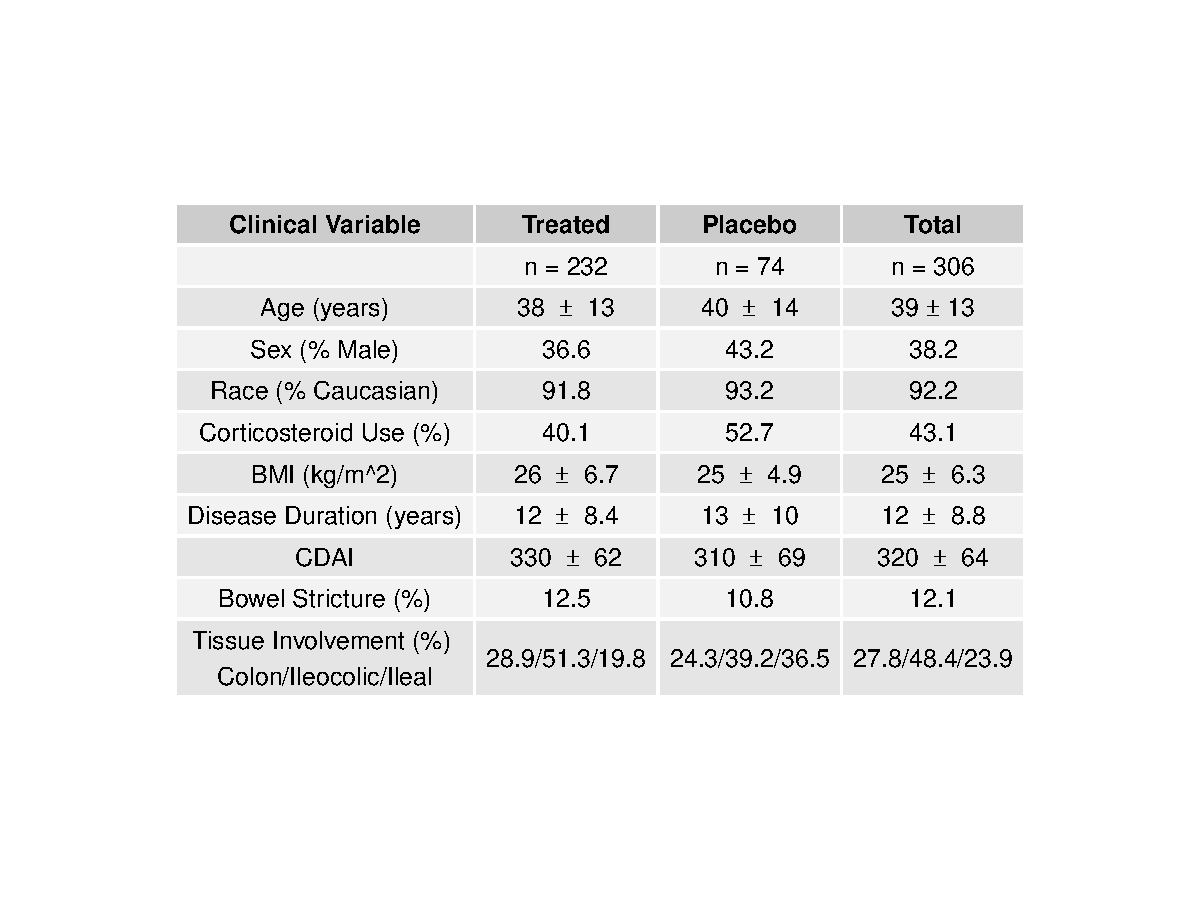
\includegraphics{tables/Table1_baseline_metadata.pdf}
\DIFaddbegin \textit{\DIFadd{No significant differences were observed between placebo and treated groups for any of the listed variables (all P>0.05).}}
\DIFaddend 

\newpage

\textbf{Table 2: Summary of subjects in each treatment group by endpoint
and outcome}

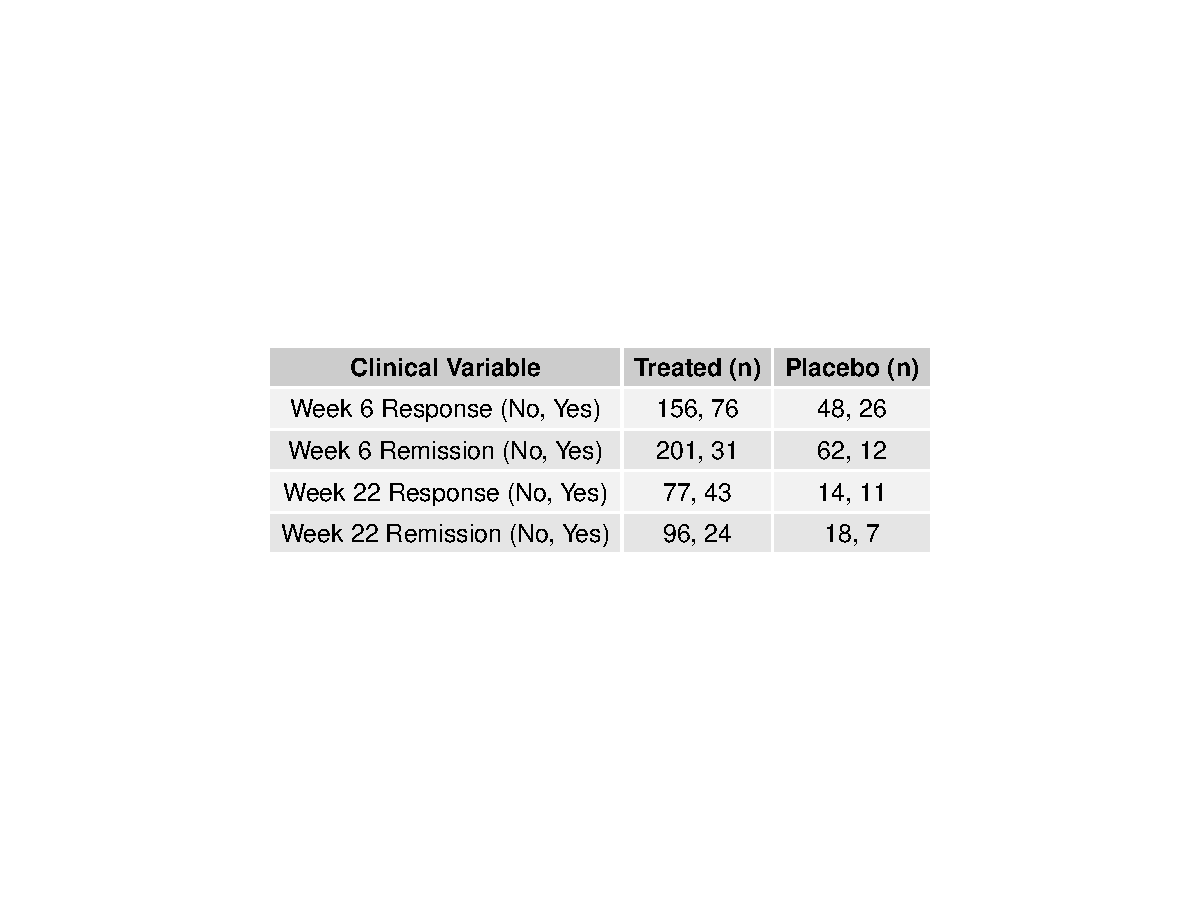
\includegraphics{tables/table2_resposne_treatN.pdf}
\DIFaddbegin 

\newpage

\textbf{\DIFadd{Table 3: Summary of microbial associations with remission at
baseline and following UST induction in treated subjects}}

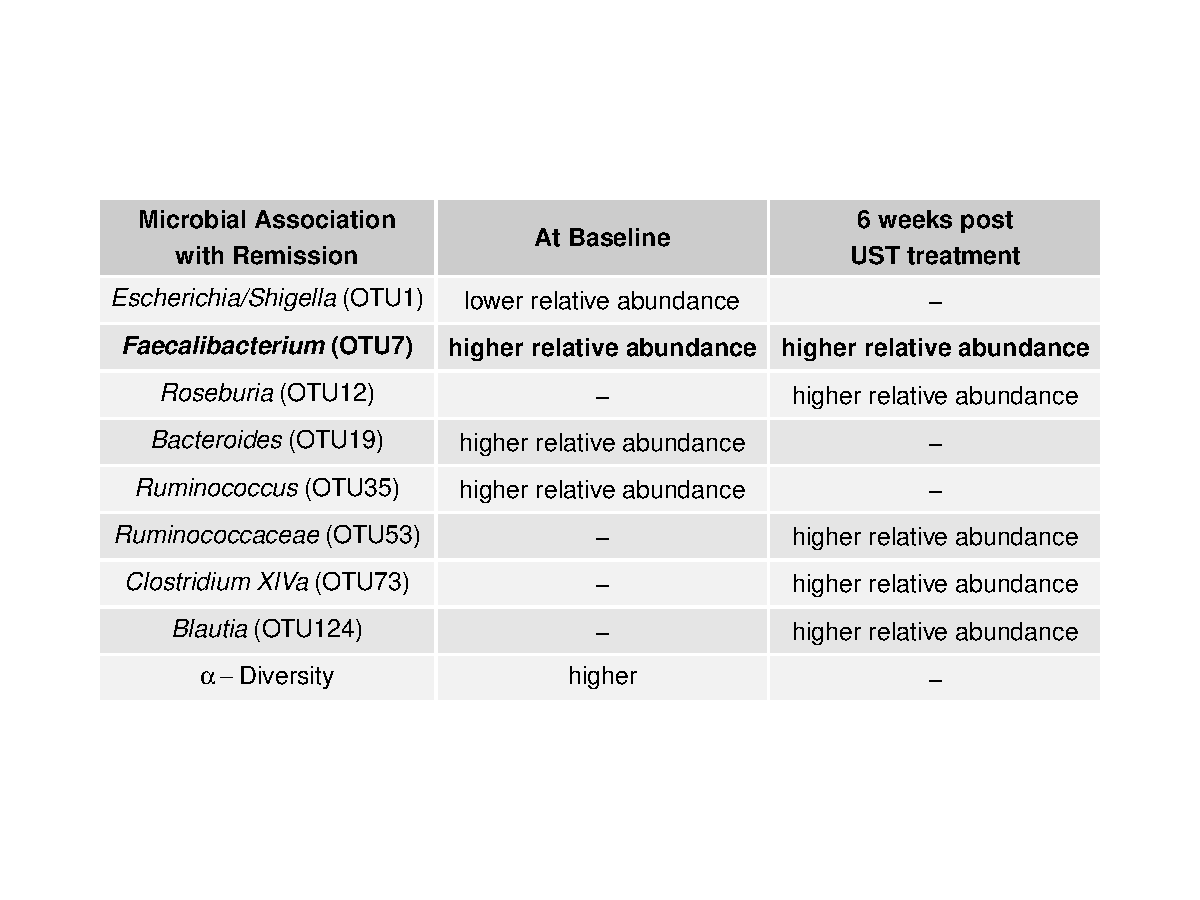
\includegraphics{tables/table3_results_table.pdf}
\DIFaddend 

\newpage

\textbf{Supplemental Table 1: Diversity differences based on clinical
metadata of cohort at baseline}

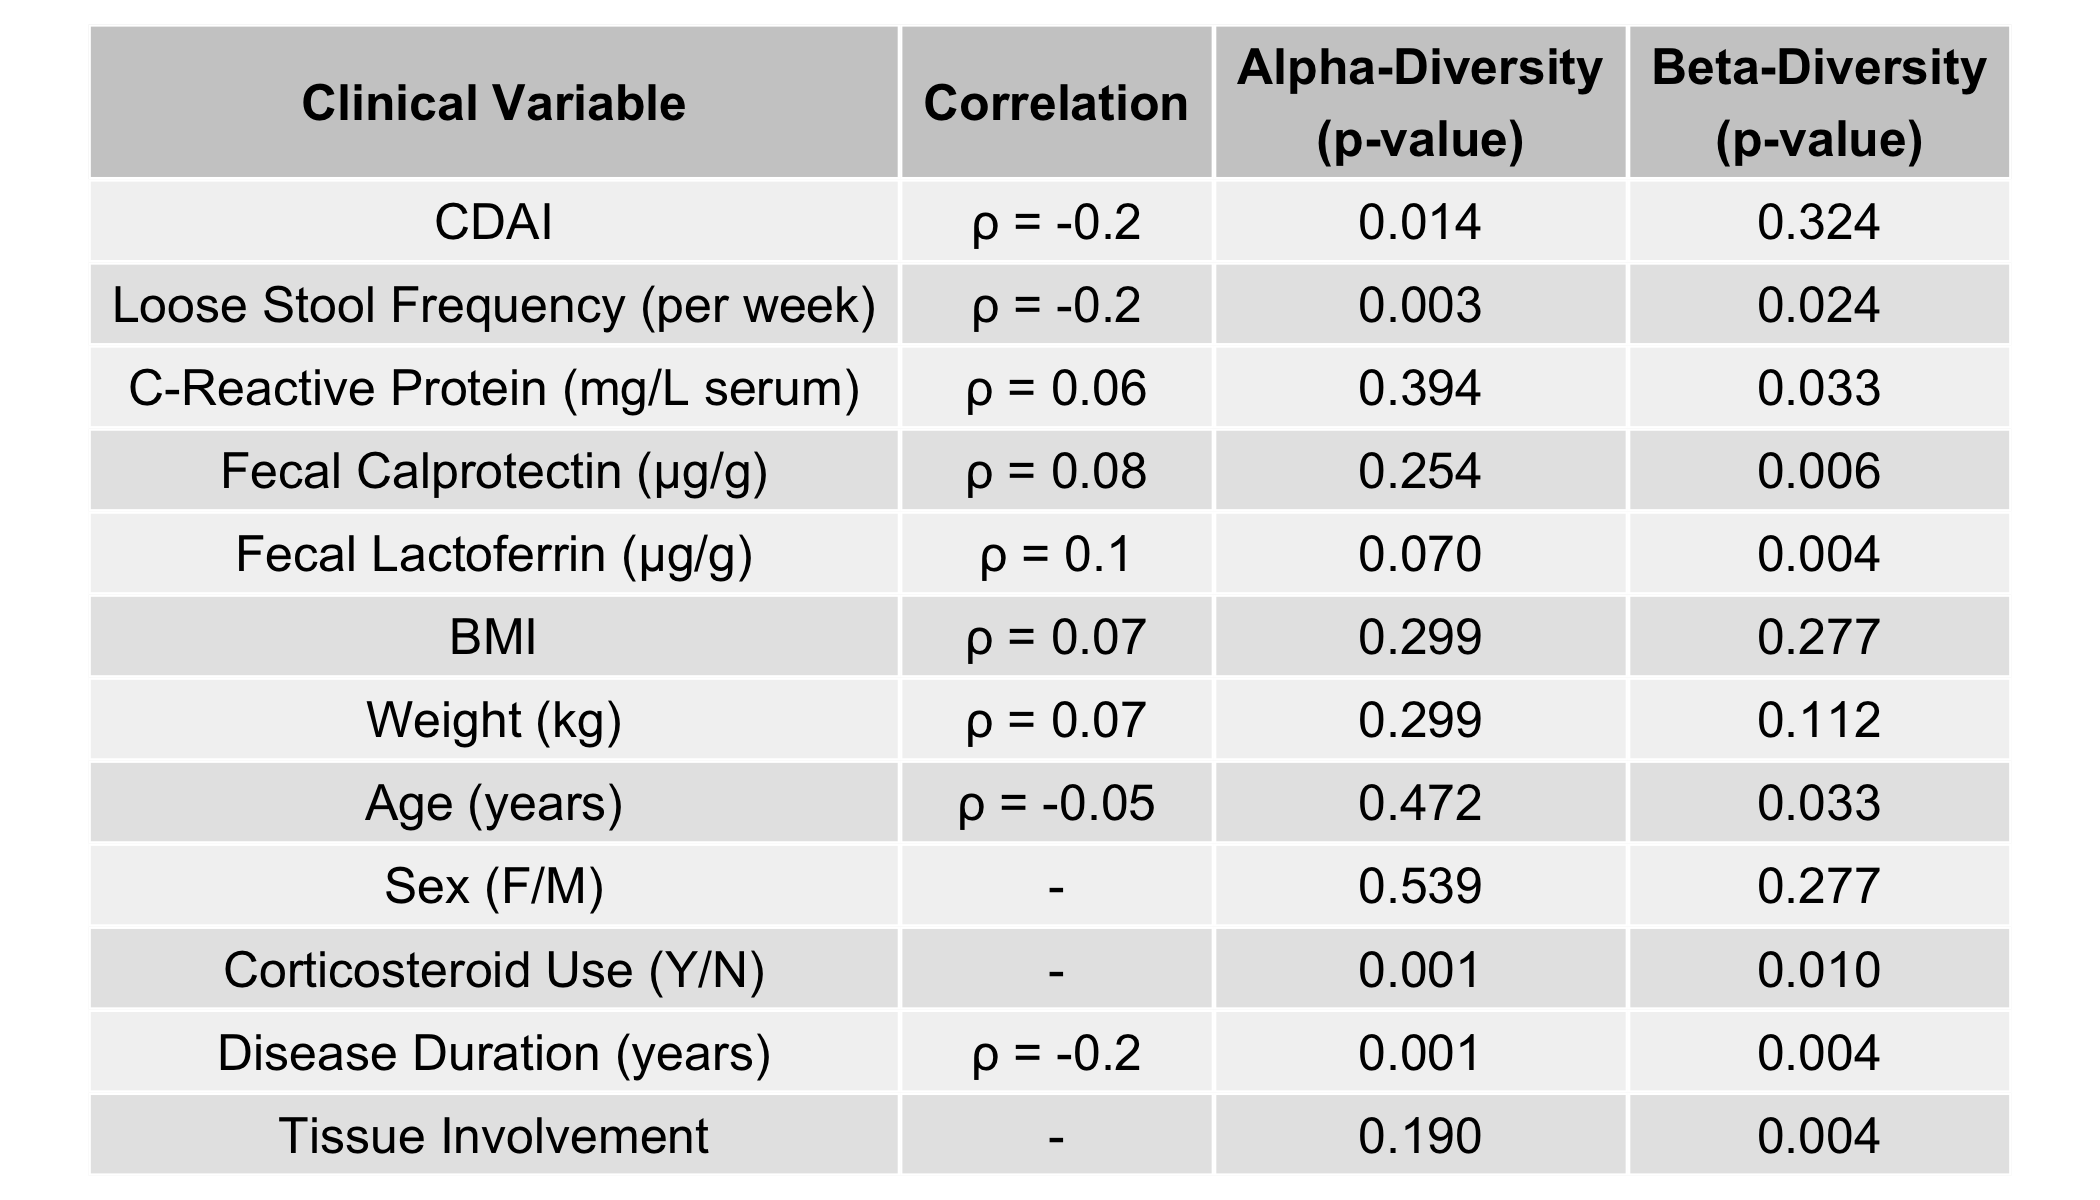
\includegraphics{tables/Supp.table1_cohortdiversity.png}

\newpage

\subsection{Figures}\label{figures}

\textbf{Figure 1: Experimental design as adapted from Sandborn et al
2012.} (A) Participants were divided into treatment groups receiving
placebo or UST by IV for induction. At week 8, subjects were divided
into groups receiving either subcutaneous injection of UST or placebo at
weeks 8 and 16 as maintenance therapy, based on response at week 6.
Finally, at 22 weeks subjects were scored using CDAI for their response
to therapy. (B) Stool sampling, treatment, and response evaluation time
line. \(\uparrow\), treatment administration; IV, intravenous; PE,
primary endpoint; R, randomization; RR, re-randomization (only for
subjects receiving UST induction therapy); SC, subcutaneous.

\textbf{Figure 2: Prediction of week 6 treatment outcome in subjects
treated with UST, using baseline samples} Receiver operating
characteristic (ROC) curves for (A) response and (C) remission using
microbiota data (blue), clinical metadata (black), and a combined model
(red). Top predictive OTUs for the microbiota model based on mean
decrease in accuracy (MDA) for (B) response and (D) remission. Black
bars represent the median relative abundance.

\textbf{Figure 3: Differential taxa in baseline stool samples from
subjects treated with UST, based on week six remission status} The
baseline relative abundance of each OTU was compared between subjects in
remission and those with active CD 6 weeks after induction using a
Wilcoxon rank sum test followed by a Benjamini-Hochberg correction for
multiple comparisons. This identified 2 OTUs with significantly
different relative abundance at baseline (p \textless{} 0.05). Black
bars represent the median relative abundance.

\textbf{Figure 4: Change in alpha diversity over time by induction
treatment and week 22 response status.} The \({\alpha}\)-diversity of 48
subjects induced and maintained with UST and 14 subjects induced and
maintained with placebo was assessed at each time point. Friedman test
were performed within each treatment and responder group. Whiskers
represent the range and boxes represent the 25-75\% interquartile range
of the median (black bar). * indicates week 22 is significantly
different from baseline (p \textless{}0.05).

\textbf{Figure 5: Classification of week 6 response or remission status
using week 6 stool samples from subjects treated with UST} (A) ROC
curves for week 6 outcome based on the week 6 microbiota. (B) Predictive
OTUs from week 6 stool for remission status at 6 weeks after induction,
based on mean decrease in accuracy. Black bars represent the median
relative abundance.

\textbf{Supplemental Figure 1: Phyla from baseline stool samples in
subjects treated with UST by week six outcome} The relative abundance of
each phylum in UST treated subjects were compared based on (A) response
and (B) remission status using a Wilcoxon rank sum test and to identify
phyla where there was a p-value less than 0.05 following a
Benjamini-Hochberg correction for multiple comparisons. No comparisons
were significant. Whiskers represent the range and boxes represent the
25-75\% interquartile range of the median (black bar).

\newpage

\section*{References}\label{references}
\addcontentsline{toc}{section}{References}

\hypertarget{refs}{}
\hypertarget{ref-Huang_gingivitis_2014}{}
1. Huang S, Li R, Zeng X, He T, Zhao H, Chang A, Bo C, Chen J, Yang F,
Knight R, Liu J, Davis C, Xu J. 2014. Predictive modeling of gingivitis
severity and susceptibility via oral microbiota. ISME J 8:1768--80.

\hypertarget{ref-Wang_cvdrisk_2016}{}
2. Wang Y, Ames NP, Tun HM, Tosh SM, Jones PJ, Khafipour E. 2016. High
molecular weight barley β-glucan alters gut microbiota toward reduced
cardiovascular disease risk. Front Microbiol 7.

\hypertarget{ref-Schubert_cdiff_2015}{}
3. Schubert AM, Sinani H, Schloss PD. 2015. Antibiotic-induced
alterations of the murine gut microbiota and subsequent effects on
colonization resistance against clostridium difficile. MBio 6:e00974.

\hypertarget{ref-Seekatz_cdiff_2016}{}
4. Seekatz AM, Rao K, Santhosh K, Young VB. 2016. Dynamics of the fecal
microbiome in patients with recurrent and nonrecurrent clostridium
difficile infection. Genome Med 8.

\hypertarget{ref-zackular_CRC_2014}{}
5. Zackular JP, Rogers MA, Ruffin MT th, Schloss PD. 2014. The human gut
microbiome as a screening tool for colorectal cancer. Cancer Prev Res
(Phila) 7:1112--21.

\hypertarget{ref-baxter_FIT_2016}{}
6. Baxter NT, Ruffin MT th, Rogers MA, Schloss PD. 2016.
Microbiota-based model improves the sensitivity of fecal immunochemical
test for detecting colonic lesions. Genome Med 8:37.

\hypertarget{ref-Klatt_microbicide_2017}{}
7. Klatt NR, Cheu R, Birse K, Zevin AS, Perner M, Noel-Romas L, Grobler
A, Westmacott G, Xie IY, Butler J, Mansoor L, McKinnon LR, Passmore JS,
Abdool Karim Q, Abdool Karim SS, Burgener AD. 2017. Vaginal bacteria
modify hiv tenofovir microbicide efficacy in african women. Science
356:938--945.

\hypertarget{ref-Haiser_cardiac_2013}{}
8. Haiser HJ, Gootenberg DB, Chatman K, Sirasani G, Balskus EP,
Turnbaugh PJ. 2013. Predicting and manipulating cardiac drug
inactivation by the human gut bacterium eggerthella lenta. Science
341:295--8.

\hypertarget{ref-Sivan_cancer_2015}{}
9. Sivan A, Corrales L, Hubert N, Williams JB, Aquino-Michaels K, Earley
ZM, Benyamin FW, Lei YM, Jabri B, Alegre ML, Chang EB, Gajewski TF.
2015. Commensal bifidobacterium promotes antitumor immunity and
facilitates anti-pd-l1 efficacy. Science 350:1084--9.

\hypertarget{ref-Vetizou_cancer_2015}{}
10. Vetizou M, Pitt JM, Daillere R, Lepage P, Waldschmitt N, Flament C,
Rusakiewicz S, Routy B, Roberti MP, Duong CP, Poirier-Colame V, Roux A,
Becharef S, Formenti S, Golden E, Cording S, Eberl G, Schlitzer A,
Ginhoux F, Mani S, Yamazaki T, Jacquelot N, Enot DP, Berard M, Nigou J,
Opolon P, Eggermont A, Woerther PL, Chachaty E, Chaput N, Robert C,
Mateus C, Kroemer G, Raoult D, Boneca IG, Carbonnel F, Chamaillard M,
Zitvogel L. 2015. Anticancer immunotherapy by ctla-4 blockade relies on
the gut microbiota. Science 350:1079--84.

\hypertarget{ref-gevers_pedsCD_2014}{}
11. Gevers D, Kugathasan S, Denson LA, Vazquez-Baeza Y, Van Treuren W,
Ren B, Schwager E, Knights D, Song SJ, Yassour M, Morgan XC, Kostic AD,
Luo C, Gonzalez A, McDonald D, Haberman Y, Walters T, Baker S, Rosh J,
Stephens M, Heyman M, Markowitz J, Baldassano R, Griffiths A, Sylvester
F, Mack D, Kim S, Crandall W, Hyams J, Huttenhower C, Knight R, Xavier
RJ. 2014. The treatment-naive microbiome in new-onset crohn's disease.
Cell Host Microbe 15:382--92.

\hypertarget{ref-wang_pedsCD_2016}{}
12. Wang F, Kaplan JL, Gold BD, Bhasin MK, Ward NL, Kellermayer R,
Kirschner BS, Heyman MB, Dowd SE, Cox SB, Dogan H, Steven B, Ferry GD,
Cohen SA, Baldassano RN, Moran CJ, Garnett EA, Drake L, Otu HH, Mirny
LA, Libermann TA, Winter HS, Korolev KS. 2016. Detecting microbial
dysbiosis associated with pediatric crohn disease despite the high
variability of the gut microbiota. Cell Rep.

\hypertarget{ref-Tew2016_UC}{}
13. Tew GW, Hackney JA, Gibbons D, Lamb CA, Luca D, Egen JG, Diehl L,
Eastham Anderson J, Vermeire S, Mansfield JC, Feagan BG, Panes J,
Baumgart DC, Schreiber S, Dotan I, Sandborn WJ, Kirby JA, Irving PM, De
Hertogh G, Van Assche GA, Rutgeerts P, O'Byrne S, Hayday A, Keir ME.
2016. Association between response to etrolizumab and expression of
integrin alphaE and granzyme a in colon biopsies of patients with
ulcerative colitis. Gastroenterology 150:477--87.e9.

\hypertarget{ref-Ananthakrishnan_IBD_2017}{}
14. Ananthakrishnan AN, Luo C, Yajnik V, Khalili H, Garber JJ, Stevens
BW, Cleland T, Xavier RJ. 2017. Gut microbiome function predicts
response to anti-integrin biologic therapy in inflammatory bowel
diseases. Cell Host Microbe 21:603--610.e3.

\hypertarget{ref-Kolho2015_pedIBD}{}
15. Kolho KL, Korpela K, Jaakkola T, Pichai MV, Zoetendal EG, Salonen A,
Vos WM de. 2015. Fecal microbiota in pediatric inflammatory bowel
disease and its relation to inflammation. Am J Gastroenterol
110:921--30.

\hypertarget{ref-Shaw_response_2016}{}
16. Shaw KA, Bertha M, Hofmekler T, Chopra P, Vatanen T, Srivatsa A,
Prince J, Kumar A, Sauer C, Zwick ME, Satten GA, Kostic AD, Mulle JG,
Xavier RJ, Kugathasan S. 2016. Dysbiosis, inflammation, and response to
treatment: A longitudinal study of pediatric subjects with newly
diagnosed inflammatory bowel disease. Genome Med 8:75.

\hypertarget{ref-ananthakrishnan_epidemiology_2015}{}
17. Ananthakrishnan AN. 2015. Epidemiology and risk factors for IBD. Nat
Rev Gastroenterol Hepatol 12:205--217.

\hypertarget{ref-floyd_economicburden_2015}{}
18. Floyd DN, Langham S, Severac HC, Levesque BG. 2015. The economic and
quality-of-life burden of crohn's disease in europe and the united
states, 2000 to 2013: A systematic review. Dig Dis Sci 60:299--312.

\hypertarget{ref-randall_CDbiologics_2015}{}
19. Randall CW, Vizuete JA, Martinez N, Alvarez JJ, Garapati KV,
Malakouti M, Taboada CM. 2015. From historical perspectives to modern
therapy: A review of current and future biological treatments for
crohn's disease. Therap Adv Gastroenterol 8:143--59.

\hypertarget{ref-wils_ust_2015}{}
20. Wils P, Bouhnik Y, Michetti P, Flourie B, Brixi H, Bourrier A, Allez
M, Duclos B, Grimaud JC, Buisson A, Amiot A, Fumery M, Roblin X,
Peyrin-Biroulet L, Filippi J, Bouguen G, Abitbol V, Coffin B, Simon M,
Laharie D, Pariente B. 2015. Subcutaneous ustekinumab provides clinical
benefit for two-thirds of patients with crohn's disease refractory to
anti-tumor necrosis factor agents. Clin Gastroenterol Hepatol.

\hypertarget{ref-colombel_deepremission_2015}{}
21. Colombel JF, Reinisch W, Mantzaris GJ, Kornbluth A, Rutgeerts P,
Tang KL, Oortwijn A, Bevelander GS, Cornillie FJ, Sandborn WJ. 2015.
Randomised clinical trial: Deep remission in biologic and
immunomodulator naive patients with crohn's disease - a SONIC post hoc
analysis. Aliment Pharmacol Ther 41:734--46.

\hypertarget{ref-baert_mucosalhealing_2010}{}
22. Baert F, Moortgat L, Van Assche G, Caenepeel P, Vergauwe P, De Vos
M, Stokkers P, Hommes D, Rutgeerts P, Vermeire S, D'Haens G. 2010.
Mucosal healing predicts sustained clinical remission in patients with
early-stage crohn's disease. Gastroenterology 138:463--8; quiz e10--1.

\hypertarget{ref-Lichtenstein_biomarkers_2010}{}
23. Lichtenstein GR. 2010. Emerging prognostic markers to determine
crohn's disease natural history and improve management strategies: A
review of recent literature. Gastroenterol Hepatol (N Y) 6:99--107.

\hypertarget{ref-Chang_biomarkers_2015}{}
24. Chang S, Malter L, Hudesman D. 2015. Disease monitoring in
inflammatory bowel disease. World J Gastroenterol 21:11246--59.

\hypertarget{ref-Boon_biomarkers_2015}{}
25. Boon GJ, Day AS, Mulder CJ, Gearry RB. 2015. Are faecal markers good
indicators of mucosal healing in inflammatory bowel disease? World J
Gastroenterol 21:11469--80.

\hypertarget{ref-Falvey_biomarkers_2015}{}
26. Falvey JD, Hoskin T, Meijer B, Ashcroft A, Walmsley R, Day AS,
Gearry RB. 2015. Disease activity assessment in ibd: Clinical indices
and biomarkers fail to predict endoscopic remission. Inflamm Bowel Dis
21:824--31.

\hypertarget{ref-sartor_IBDpath_2006}{}
27. Sartor RB. 2006. Mechanisms of disease: Pathogenesis of crohn's
disease and ulcerative colitis. Nat Clin Pract Gastroenterol Hepatol
3:390--407.

\hypertarget{ref-wright_CDmicrobiome_2015}{}
28. Wright EK, Kamm MA, Teo SM, Inouye M, Wagner J, Kirkwood CD. 2015.
Recent advances in characterizing the gastrointestinal microbiome in
crohn's disease: A systematic review. Inflamm Bowel Dis 21:1219--28.

\hypertarget{ref-manichanh_diversityCD_2006}{}
29. Manichanh C, Rigottier-Gois L, Bonnaud E, Gloux K, Pelletier E,
Frangeul L, Nalin R, Jarrin C, Chardon P, Marteau P, Roca J, Dore J.
2006. Reduced diversity of faecal microbiota in crohn's disease revealed
by a metagenomic approach. Gut 55:205--11.

\hypertarget{ref-hansen_pedsIBD_2012}{}
30. Hansen R, Russell RK, Reiff C, Louis P, McIntosh F, Berry SH,
Mukhopadhya I, Bisset WM, Barclay AR, Bishop J, Flynn DM, McGrogan P,
Loganathan S, Mahdi G, Flint HJ, El-Omar EM, Hold GL. 2012. Microbiota
of de-novo pediatric IBD: Increased faecalibacterium prausnitzii and
reduced bacterial diversity in crohn's but not in ulcerative colitis. Am
J Gastroenterol 107:1913--22.

\hypertarget{ref-haberman_pedsCD_2014}{}
31. Haberman Y, Tickle TL, Dexheimer PJ, Kim MO, Tang D, Karns R,
Baldassano RN, Noe JD, Rosh J, Markowitz J, Heyman MB, Griffiths AM,
Crandall WV, Mack DR, Baker SS, Huttenhower C, Keljo DJ, Hyams JS,
Kugathasan S, Walters TD, Aronow B, Xavier RJ, Gevers D, Denson LA.
2014. Pediatric crohn disease patients exhibit specific ileal
transcriptome and microbiome signature. J Clin Invest 124:3617--33.

\hypertarget{ref-Riol-Blanco_IL23microbiome_2010}{}
32. Riol-Blanco L, Lazarevic V, Awasthi A, Mitsdoerffer M, Wilson BS,
Croxford A, Waisman A, Kuchroo VK, Glimcher LH, Oukka M. 2010. IL-23
receptor regulates unconventional il-17-producing t cells that control
infection1. J Immunol 184:1710--20.

\hypertarget{ref-Round_IL23microbiome_2009}{}
33. Round JL, Mazmanian SK. 2009. The gut microbiome shapes intestinal
immune responses during health and disease. Nat Rev Immunol 9:313--23.

\hypertarget{ref-Eken_IL23CD_2014}{}
34. Eken A, Singh AK, Oukka M. 2014. INTERLEUKIN 23 in crohn'S disease.
Inflamm Bowel Dis 20:587--95.

\hypertarget{ref-Shih_IL23Th17_2014}{}
35. Shih VFS, Cox J, Kljavin NM, Dengler HS, Reichelt M, Kumar P,
Rangell L, Kolls JK, Diehl L, Ouyang W, Ghilardi N. 2014. Homeostatic
il-23 receptor signaling limits th17 response through il-22--mediated
containment of commensal microbiota. Proc Natl Acad Sci U S A
111:13942--7.

\hypertarget{ref-tedjo_CDactivity_2016}{}
36. Tedjo DI, Smolinska A, Savelkoul PH, Masclee AA, Schooten FJ van,
Pierik MJ, Penders J, Jonkers DMAE. 2016. The fecal microbiota as a
biomarker for disease activity in crohn's disease. Scientific Reports,
Published online: 13 October 2016; doi:101038/srep35216.

\hypertarget{ref-sandborn_ust_2012}{}
37. Sandborn WJ, Gasink C, Gao LL, Blank MA, Johanns J, Guzzo C, Sands
BE, Hanauer SB, Targan S, Rutgeerts P, Ghosh S, Villiers WJ de,
Panaccione R, Greenberg G, Schreiber S, Lichtiger S, Feagan BG. 2012.
Ustekinumab induction and maintenance therapy in refractory crohn's
disease. N Engl J Med 367:1519--28.

\hypertarget{ref-sandborn_ust_2008}{}
38. Sandborn WJ, Feagan BG, Fedorak RN, Scherl E, Fleisher MR, Katz S,
Johanns J, Blank M, Rutgeerts P. 2008. A randomized trial of
ustekinumab, a human interleukin-12/23 monoclonal antibody, in patients
with moderate-to-severe crohn's disease. Gastroenterology 135:1130--41.

\hypertarget{ref-kopylov_ust_2014}{}
39. Kopylov U, Afif W, Cohen A, Bitton A, Wild G, Bessissow T, Wyse J,
Al-Taweel T, Szilagyi A, Seidman E. 2014. Subcutaneous ustekinumab for
the treatment of anti-TNF resistant crohn's disease--the McGill
experience. J Crohns Colitis 8:1516--22.

\hypertarget{ref-PB_CDAI_2016}{}
40. Peyrin-Biroulet L, Panes J, Sandborn WJ, Vermeire S, Danese S,
Feagan BG, Colombel JF, Hanauer SB, Rycroft B. 2016. Defining disease
severity in inflammatory bowel diseases: Current and future directions.
Clin Gastroenterol Hepatol 14:348--354.e17.

\hypertarget{ref-Best_CDAI_1976}{}
41. Best WR, Becktel JM, Singleton JW, Kern J F. 1976. Development of a
crohn's disease activity index. national cooperative crohn's disease
study. Gastroenterology 70:439--44.

\hypertarget{ref-calle_aucrf_2011}{}
42. Calle ML, Urrea V, Boulesteix A-L, Malats N. 2011. AUC-RF: A new
strategy for genomic profiling with random forest. Human Heredity
72:121--132.

\hypertarget{ref-Vogenberg_progmods_2009}{}
43. Vogenberg FR. 2009. Predictive and prognostic models: Implications
for healthcare decision-making in a modern recession. Am Health Drug
Benefits 2:218--22.

\hypertarget{ref-naftali_tissinvol_2016}{}
44. Naftali T, Reshef L, Kovacs A, Porat R, Amir I, Konikoff FM, Gophna
U. 2016. Distinct microbiotas are associated with ileum-restricted and
colon-involving crohn's disease. Inflamm Bowel Dis 22:293--302.

\hypertarget{ref-sartor_microbesIBD_2016}{}
45. Sartor RB, Wu GD. 2016. Roles for intestinal bacteria, viruses, and
fungi in pathogenesis of inflammatory bowel diseases and therapeutic
approaches. Gastroenterology.

\hypertarget{ref-Williet2014_PROs}{}
46. Williet N, Sandborn WJ, Peyrin-Biroulet L. 2014. Patient-reported
outcomes as primary end points in clinical trials of inflammatory bowel
disease. Clin Gastroenterol Hepatol 12:1246--56.e6.

\hypertarget{ref-boon_fmarkers_2015}{}
47. Boon GJ, Day AS, Mulder CJ, Gearry RB. 2015. Are faecal markers good
indicators of mucosal healing in inflammatory bowel disease? World J
Gastroenterol 21:11469--80.

\hypertarget{ref-chang_monitoring_2015}{}
48. Chang S, Malter L, Hudesman D. 2015. Disease monitoring in
inflammatory bowel disease. World J Gastroenterol 21:11246--59.

\hypertarget{ref-papa_pedsIBD_2012}{}
49. Papa E, Docktor M, Smillie C, Weber S, Preheim SP, Gevers D,
Giannoukos G, Ciulla D, Tabbaa D, Ingram J, Schauer DB, Ward DV,
Korzenik JR, Xavier RJ, Bousvaros A, Alm EJ. 2012. Non-invasive mapping
of the gastrointestinal microbiota identifies children with inflammatory
bowel disease. PLoS One 7:e39242.

\hypertarget{ref-vandeputte_stoolcon_2016}{}
50. Vandeputte D, Falony G, Vieira-Silva S, Tito RY, Joossens M, Raes J.
2016. Original article: Stool consistency is strongly associated with
gut microbiota richness and composition, enterotypes and bacterial
growth rates. Gut 65:57--62.

\hypertarget{ref-huang_cort_2015}{}
51. Huang EY, Inoue T, Leone VA, Dalal S, Touw K, Wang Y, Musch MW,
Theriault B, Higuchi K, Donovan S, Gilbert J, Chang EB. 2015. Using
corticosteroids to reshape the gut microbiome: Implications for
inflammatory bowel diseases. Inflamm Bowel Dis 21:963--72.

\hypertarget{ref-schloss_mothur_2009}{}
52. Schloss PD, Westcott SL, Ryabin T, Hall JR, Hartmann M, Hollister
EB, Lesniewski RA, Oakley BB, Parks DH, Robinson CJ, Sahl JW, Stres B,
Thallinger GG, Van Horn DJ, Weber CF. 2009. Introducing mothur:
Open-source, platform-independent, community-supported software for
describing and comparing microbial communities. Appl Environ Microbiol
75:7537--41.

\hypertarget{ref-Kozich_MiSeqSOP_2013}{}
53. Kozich JJ, Westcott SL, Baxter NT, Highlander SK, Schloss PD. 2013.
Development of a dual-index sequencing strategy and curation pipeline
for analyzing amplicon sequence data on the miseq illumina sequencing
platform. Appl Environ Microbiol 79:5112--20.

\hypertarget{ref-schloss_PCRartifacts_2011}{}
54. Schloss PD, Gevers D, Westcott SL. 2011. Reducing the effects of PCR
amplification and sequencing artifacts on 16S rRNA-based studies. PLoS
One 6:e27310.

\hypertarget{ref-Quast_silva_2013}{}
55. Quast C, Pruesse E, Yilmaz P, Gerken J, Schweer T, Yarza P, Peplies
J, Glöckner FO. 2013. The silva ribosomal rna gene database project:
Improved data processing and web-based tools. Nucleic Acids Res
41:D590--6.

\hypertarget{ref-edgar_uchime_2011}{}
56. Edgar RC, Haas BJ, Clemente JC, Quince C, Knight R. 2011. UCHIME
improves sensitivity and speed of chimera detection. Bioinformatics
27:2194--200.

\hypertarget{ref-schloss_OTUanalysis_2011}{}
57. Schloss PD, Westcott SL. 2011. Assessing and improving methods used
in operational taxonomic unit-based approaches for 16S rRNA gene
sequence analysis. Appl Environ Microbiol 77:3219--26.

\hypertarget{ref-wang_taxonomy_2007}{}
58. Wang Q, Garrity GM, Tiedje JM, Cole JR. 2007. Naive bayesian
classifier for rapid assignment of rRNA sequences into the new bacterial
taxonomy. Appl Environ Microbiol 73:5261--7.

\hypertarget{ref-R}{}
59. R Core Team. 2016. R: A language and environment for statistical
computing. R Foundation for Statistical Computing, Vienna, Austria.

\hypertarget{ref-sokal_biometrystats_1995}{}
60. Sokal RR, Rohlf FJ. 1995. Biometry: The principles and practice of
statistics in biological research, 3rd ed. Freeman, New York.

\hypertarget{ref-magurran_measuring_2004}{}
61. Magurran AE. 2004. Measuring biological diversity. Blackwell Pub.,
Malden, Ma.

\hypertarget{ref-yue_thetaYC_2005}{}
62. Yue JC, Clayton MK. 2005. A similarity measure based on species
proportions. Communications in Statistics-Theory and Methods
34:2123--2131.

\hypertarget{ref-oksanen_vegan_2016}{}
63. Oksanen J, Blanchet FG, Friendly M, Kindt R, Legendre P, McGlinn D,
Minchin PR, O'Hara RB, Simpson GL, Solymos P, Stevens MHH, Szoecs E,
Wagner H. 2016. Vegan: Community ecology package. r package version
2.4-1.

\hypertarget{ref-friedman_1937}{}
64. Friedman M. 1937. The use of ranks to avoid the assumption of
normality implicit in the analysis of variance. Journal of the American
Statistical Association 32:675--701.

\hypertarget{ref-pgirmess}{}
65. Giraudoux P. 2016. Pgirmess: Data analysis in ecology.

\hypertarget{ref-AUCRF}{}
66. Urrea V, Calle M. 2012. AUCRF: Variable selection with random forest
and the area under the curve.

\hypertarget{ref-breiman_rf_2001}{}
67. Breiman L. 2001. Random forests. Machine Learning 45:5--32.

\hypertarget{ref-Benjamini_Hochberg_1995}{}
68. Benjamini Y, Hochberg Y. 1995. Controlling the false discovery rate:
A practical and powerful approach to multiple testing. Journal of the
Royal Statistical Society Series B (Methodological) 57:289--300.

\hypertarget{ref-ggplot2}{}
69. Wickham H. 2009. Ggplot2: Elegant graphics for data analysis.
Springer-Verlag New York.

\hypertarget{ref-dplyr}{}
70. Wickham H, Francois R. 2016. Dplyr: A grammar of data manipulation.

\hypertarget{ref-pROC}{}
71. Robin X, Turck N, Hainard A, Tiberti N, Lisacek F, Sanchez J-C,
Müller M. 2011. PROC: An open-source package for r and s+ to analyze and
compare roc curves. BMC Bioinformatics 12:77.

\hypertarget{ref-knitr2015}{}
72. Xie Y. 2015. Dynamic documents with R and knitr, 2nd ed. Chapman;
Hall/CRC, Boca Raton, Florida.

\hypertarget{ref-gridExtra}{}
73. Auguie B. 2016. GridExtra: Miscellaneous functions for ``grid''
graphics.

\hypertarget{ref-devtools}{}
74. Wickham H, Chang W. 2016. Devtools: Tools to make developing r
packages easier.

\hypertarget{ref-knitcitations}{}
75. Boettiger C. 2015. Knitcitations: Citations for 'knitr' markdown
files.

\hypertarget{ref-scales}{}
76. Wickham H. 2016. Scales: Scale functions for visualization.

\hypertarget{ref-tidyr}{}
77. Wickham H. 2017. Tidyr: Easily tidy data with 'spread()' and
'gather()' functions.

\hypertarget{ref-Hmisc}{}
78. Harrell Jr FE, Charles Dupont, others. 2016. Hmisc: Harrell
miscellaneous.

\hypertarget{ref-cowplot}{}
79. Wilke CO. 2016. Cowplot: Streamlined plot theme and plot annotations
for 'ggplot2'.


\end{document}
